\chapter{Parameter Selection}
\label{ch:parameterSelection}

This chapter records the tuning parameter process and why to choose them.

\section{Random Forest}
For random forest, the parameter is to tune the trees number. The following test is based on different number. Fig~\ref{fg:rtMseDF} shows MSE, fig~\ref{fg:rtCdcDF} shows CDC, and fig~\ref{fg:rtRunTimeDF} shows running time.

\begin{figure}[h]
	\centering
	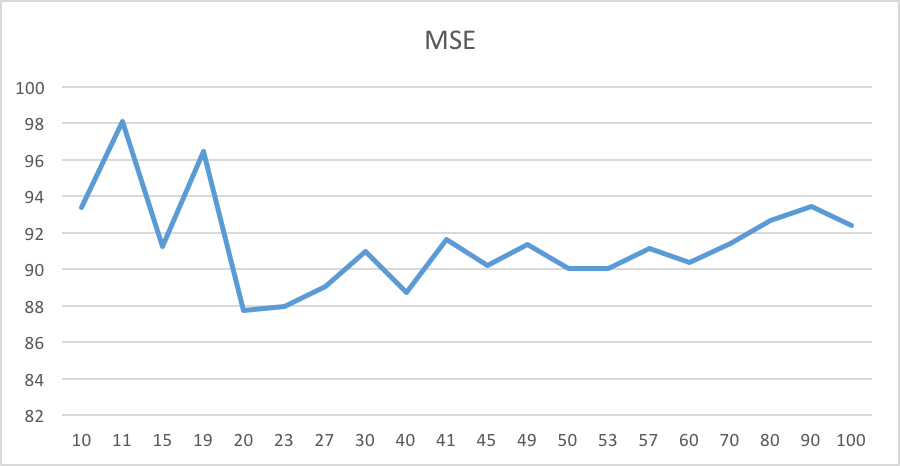
\includegraphics[width=0.8\textwidth]{FeatureSelection/rtMse}
	\caption{The average MSE result vs different random forest tree number}
	\label{fg:rtMseDF}
\end{figure}

\begin{figure}[h]
	\centering
	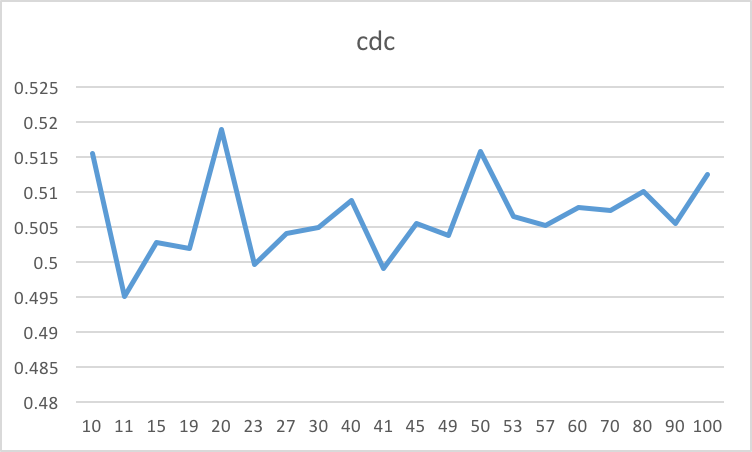
\includegraphics[width=0.8\textwidth]{FeatureSelection/rtCdc}
	\caption{The average CDC result vs different random forest tree number}
	\label{fg:rtCdcDF}
\end{figure}

\begin{figure}[h]
\centering
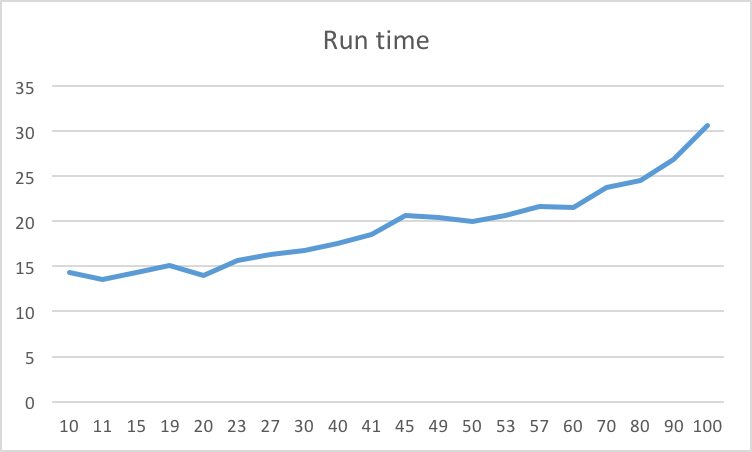
\includegraphics[width=0.8\textwidth]{FeatureSelection/rtRunTime}
\caption{The average running time result vs different random forest tree number}
\label{fg:rtRunTimeDF}
\end{figure}

From the above figures we can find that, trees number 20 is a good point as it has almost the lowest MSE and highest CDC. As the trees number increases, the running time also increases. So in the following test, the trees number will set to 20.

\section{Artificial Neural Network}
For random forest, the parameter is to tune the hidden nodes number. The following test is based on different number. Fig~\ref{fg:annMseDF} shows MSE, fig~\ref{fg:annCdcDF} shows CDC, and fig~\ref{fg:annRunTimeDf} shows running time.

\begin{figure}[h]
	\centering
	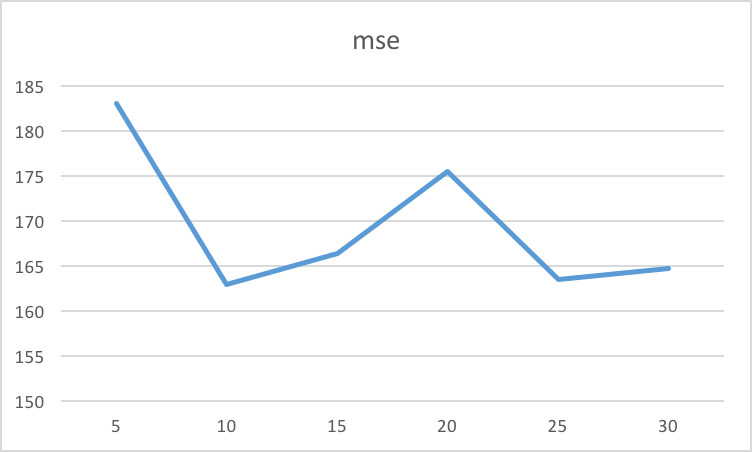
\includegraphics[width=0.8\textwidth]{FeatureSelection/annMse}
	\caption{The average MSE result vs different hidden nodes number}
	\label{fg:annMseDF}
\end{figure}

\begin{figure}[h]
	\centering
	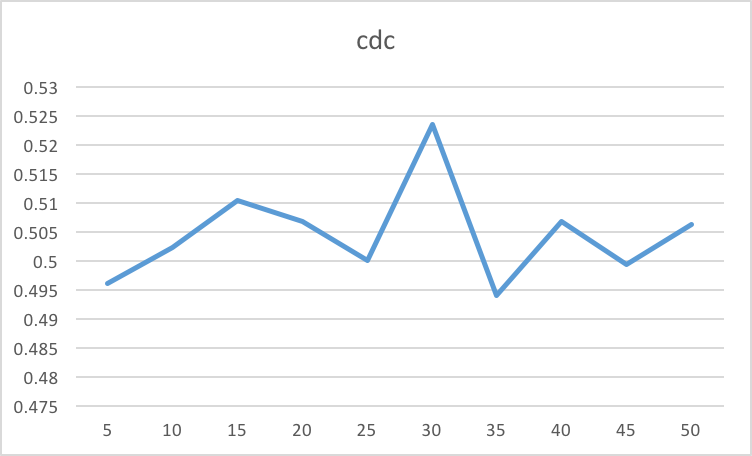
\includegraphics[width=0.8\textwidth]{FeatureSelection/annCdc}
	\caption{The average CDC result vs different hidden nodes number}
	\label{fg:annCdcDF}
\end{figure}

\begin{figure}[h]
	\centering
	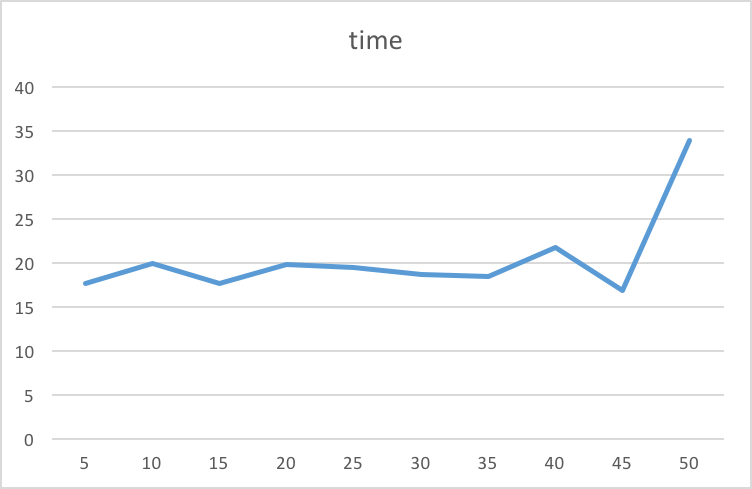
\includegraphics[width=0.8\textwidth]{FeatureSelection/annTime}
	\caption{The average running time result vs different hidden nodes number}
	\label{fg:annRunTimeDf}
\end{figure}

From the above figures we can find that, hidden nodes number 30 is a good point as it has almost the lowest MSE and highest CDC. As the trees number increases, the running time also increases. So in the following test, the hidden nodes number will set to 30.


\section{Window Size}
The window size is also needed to be determined, The test is based on above result and its results are shown in table~\ref{fg:windowSizeCDC}, \ref{fg:windowSizeMSE} and \ref{fg:windowSizeRunTime}, respectively.\\

\begin{table}[h]
	\centering
	\begin{tabular}{|c|c|c|c|c|}
		\hline
		\textbf{CDC} & \textbf{1} & \textbf{3}       & \textbf{6}       & \textbf{None} \\ \hline
		\textbf{ANN} & 50.59\%    & 50.90\%          & \textbf{51.10\%} & 51.03\%       \\ \hline
		\textbf{LRR} & 50.38\%    & 50.11\%          & \textbf{51.74\%} & 5058\%        \\ \hline
		\textbf{RT}  & 50.44\%    & \textbf{51.02\%} & 50.97\%          & 50.85\%       \\ \hline
	\end{tabular}
	\caption{Window size test CDC result}
	\label{fg:windowSizeCDC}
\end{table}

\begin{table}[h]
	\centering
	\begin{tabular}{|l|l|l|l|l|}
		\hline
		\multicolumn{1}{|c|}{\textbf{MSE}} & \multicolumn{1}{c|}{\textbf{1}} & \multicolumn{1}{c|}{\textbf{3}} & \multicolumn{1}{c|}{\textbf{6}} & \multicolumn{1}{c|}{\textbf{None}} \\ \hline
		\textbf{ANN}                       & 1.96                            & 1.91                            & 1.97                            & \textbf{1.87}                      \\ \hline
		\textbf{LRR}                       & 2.06                            & 1.98                            & \textbf{1.85}                   & 1.92                               \\ \hline
		\textbf{RT}                        & 1.87                            & \textbf{1.84}                   & 2.12                            & 1.86                               \\ \hline
	\end{tabular}
	\caption{Window size test MSE result}
	\label{fg:windowSizeMSE}
\end{table}

\begin{table}[h]
	\centering
	\begin{tabular}{|c|c|c|c|c|}
		\hline
		\textbf{Time} & \textbf{1} & \textbf{3} & \textbf{6} & \textbf{None} \\ \hline
		\textbf{ANN}  & 77.15      & 23.39      & 14.50      & \textbf{7.20} \\ \hline
		\textbf{LRR}  & 56.64      & 19.04      & 10.89      & \textbf{5.15} \\ \hline
		\textbf{RT}   & 79.38      & 24.78      & 14.23      & \textbf{6.75} \\ \hline
	\end{tabular}
	\caption{Window size test run time result}
	\label{fg:windowSizeRunTime}
\end{table}


From those results we can find that The computation time increases linearly as the window size decreases, but MSE and CDC do not change significantly. In order to balance the efficiency and effectiveness of this experiment will use all the window size of \textbf{6} to carry out.


\section{Summary}
To sum up, in this dissertation, the parameters will be set to those values:
\begin{itemize}
	\item \textbf{Random Trees Number}: 20
	\item \textbf{Artificial Neural Network Hidden Nodes Number}: 30
	\item \textbf{Window Size}: Six Month.
\end{itemize}
